\documentclass{article}
\usepackage[utf8]{inputenc}
\usepackage[margin=1in]{geometry}

\title{Textual Genre Discrimination with Dynamic Syntactic Features}
\author{Victor Zhang}
\date{December 18, 2021}

\usepackage[utf8]{inputenc}
\usepackage{amsmath}
\usepackage{amsfonts}
\usepackage{graphicx}
% \usepackage{changepage}
\usepackage{amssymb}
\usepackage{xfrac}
% \usepackage{bm}
% \usepackage{empheq}
\usepackage{dirtytalk}
\usepackage{subcaption}
\usepackage[title]{appendix}
\usepackage[square,numbers]{natbib}
\usepackage{url}
\usepackage{cleveref}
\bibliographystyle{abbrvnat}

\newcommand{\contra}{\raisebox{\depth}{\#}}

\newenvironment{myindentpar}[1]
  {\begin{list}{}
          {
            \setlength{\leftmargin}{#1}
            \setlength{\rightmargin}{#1}
          }
          \item[]
  }
  {\end{list}}

\pagestyle{empty}

\begin{document}

\maketitle
% \begin{center}
% {\huge Econ 482 \hspace{0.5cm} HW 3}\
% {\Large \textbf{Victor Zhang}}\
% {\Large February 18, 2020}
% \end{center}

\begin{abstract}
Textual genre discrimination is a prerequisite to many interesting applications in industry, including classification and higher-order NLP tasks. Much of the focus in recent years has been on static textual analysis, that is, looking at the text as a whole. We present a novel dynamic approach that trains a Markov model on part-of-speech transitions. We evaluate its efficacy on genres taken from the Brown Corpus and conclude part-of-speech Markov models are useful for determining voice and lexical complexity in addition to genre.
\end{abstract}

\section{Introduction}
Textual genre discrimination is an important preprocessing task for many industrial and research applications, including classification, retrieval, and higher-order NLP tasks \cite{LeeMyaeng}. The bulk of the current literature has focused on offline methods, that is, using only the text and insights gathered from the text to perform classification. Even still, the state of the art achieves an accuracy rate of around 92\% \cite{SoA}. Many classification schemes focus on low-level textual features (sentence length, word length) or lexical features (occurrence rate of common words, noun-to-verb ratio)\cite{KitchSink}. Very little analysis has been done on syntactic features. These features include depth of sentence parse trees, arity of verbal predicates, or dependency link lengths \cite{Italian}. Whereas these are the highest-level features explored by AI efforts, these are usually the lowest-level features considered by humans making the same classifications. We thus postulate that syntactic features represent a wealth of untapped potential for accurate classification schemes.

In this paper, we focus our attention on \textit{part of speech tags} (POS tags). In linguistics, POS combinations are a syntactic feature that represents patterns in language. For instance, an auxiliary verb followed by a participle represents a phrase in the passive voice \cite{POS} \cite{LingAuto}. POS tagging thus allows researchers to examine the structure of the text in the same way that figured bass allows musicians to examine the structure of a piece of music.

Indeed, as seen in the passive voice example, text is not static. When authoring a work, the flow of words and ideas is tantamount to the author and thus should also be considered for a genre discrimination task. So far the work in genre discrimination has treated text as nothing more than a bar chart of word frequencies or feature dumps. We argue this is an overly reductive view of writing that loses a lot of the nuance that can be recovered by looking at the text as a temporal object.

In this paper, we explore genre discrimination with part-of-speech tags and the natural temporal process that a tagged work of literature induces. We use a Markov model to capture this process and evaluate its fitness on the \textit{learned}, \textit{lore}, \textit{romance}, and \textit{mystery} genres from the Brown Corpus of Standard American English \cite{Brown} \cite{BrownManual}.

\subsection{Goals and Hypothesized Outcomes}
We aim to offer an explainable method of textual genre discrimination using methods inspired by manual genre discrimination. Ideally the finished product will involve some form of temporal model on one or more syntactic features. We hypothesize that our model will perform reasonably well, since it will rely on linguistically significant features. However, we expect to not beat the state of the art, since those methods have been refined through many years of study in academia and industry.

In the development and evaluation of this paper, we will at all times keep in mind the principles of \textit{explainability} and \textit{data bias}. Our models should also be as explainable as the human methods we draw upon for inspiration. Model decisions will be intentional and reasonable given the data presented. We will likely avoid neural networks as a whole since they are difficult to interpret and reason about. Moreover, since our evaluation hinges on the dataset we choose, it is imperative we understand the data and any biases it contains. This means a close analysis of the texts included in the corpus, both manually and with data scientific methods. Ideally, the data we pass to our models will be clean and free of confounding correlations.

\subsection{Paper Organization}
The organization of this report is as follows. Section 2 describes the dataset and preprocessing in detail, followed by technical descriptions of the Markov model and a subgenre classification study on the \textit{learned} genre. Section 3 presents results from this subgenre classification, Markov models, and a case study based on conclusions drawn from the subgenre classification. Section 4 summarizes our results and provides some possible directions for future work.

\section{Data and Methods}
\subsection{Data and Preprocessing}
For our experiments, we use the Brown Corpus, one of the earliest corpora of annotated texts and one which is available on kaggle.com with a registered account. The Brown Corpus contains 1 million words comprising 500 text samples, all produced or published in 1961. On average, a text sample is between 10-25 paragraphs and each paragraph consists of between 4-7 sentences. The texts are taken from 15 labelled genres \cite{BrownManual}. The genre breakdown is given in figure 1.
\begin{figure}[ht!]
\centering
\begin{subfigure}[T]{0.3\linewidth}
\begin{tabular}{|c|c|}
\hline
News & 44\\
\hline
Editorial & 27\\
\hline
Reviews & 30\\
\hline
Religion & 5\\
\hline
Skills and Hobbies & 36\\
\hline
Popular Lore & 48\\
\hline
Belle Lettres & 75\\
\hline
Government Documents & 30\\
\hline
Learned & 80\\
\hline
\end{tabular}
\end{subfigure}
\begin{subfigure}[T]{0.3\linewidth}
\begin{tabular}{|c|c|}
\hline
General Fiction & 29\\
\hline
Mystery and Detective & 24\\
\hline
Science Fiction & 6\\
\hline
Adventure and Western & 29\\
\hline
Romance and Love & 29\\
\hline
Humor & 9\\
\hline
\end{tabular}
\end{subfigure}
\caption{Brown corpus genre split}
\end{figure}

Each word or symbol in the corpus is also associated with a classifier representing its part of speech. In total, the Brown corpus uses over 150 distinct part-of-speech (POS) tags \cite{BrownManual}. This offers computational linguists a huge library of very nuanced tags to work with. However, for the purposes of training a Markov model, such a large tagset is unwieldy and often unnecessary. Recently, Petrov, Das, and McDonald showed that unsupervised NLP tasks can be accomplished with similar accuracy using a much smaller tagset \cite{Universal}. Their so-called \textit{universal tagset} contains just 12 tags and thus is much more suited to our goals. This reduces the nuance expressed through POS tagging but not by enough to affect model performance. As such, we may justify using the universal tagset in our Markov models.

We convert the Brown tags to universal using the mapping published as a part of the NLTK corpora \cite{NLTK}. Tags that were unmappable by automation we mapped manually. Nonsense tags were assigned the tag \verb|X| representing \say{other}. Finally, we split the tagged samples by genre.

\subsection{Sub-classification Within Genre}
Each text sample is assigned a genre by the corpus, but it is not unlikely that there are distinctive sub-genres within each genre that would complicate a classification algorithm. In particular, we were concerned about the \say{learned} genre, which includes academic writing from many disparate fields. It could be the case, for instance, that scientific writing is very different from humanities writing from the perspective of POS distribution. After all, this is true from a human perspective. Scientific writing usually uses simpler sentences and is very matter of fact while humanities writing, particularly philisophical writing, is denser and more elaborate; the cognitive complexity of scientific writing is borne by the reader whereas in philosophical writing it is borne by the text. With this in mind, we set out to find whether these percepted differences were reflected by the POS tagging. This is accomplished with a $k$-means analysis over the texts in the genre.

We transform every text into a frequency vector as follows: Represent text $x$ as a sequence $x_1, x_2, \dots, x_n$ of POS tags. Examining the transitions $x_i,x_{i+1}$, generate a 12 by 12 matrix $A$ where $A_{ij}$ represents the number of observed transitions from the $i$-th POS tag to the $j$-th. From this, generate a normalized vector
$$v'_x = (\frac{1}{n - 1}A_{1,1}, \frac{1}{n - 1}A_{1,2}, \dots, \frac{1}{n - 1}A_{1,12}, \frac{1}{n - 1}A_{2,1}, \dots, \frac{1}{n - 1}A_{12,12})$$
As previously mentioned, the 12th tag in the universal tagset is \verb|X|, representing unknown or other parts of speech. Since there are comparatively few instances of this tag compared to every other tag (roughly 250 compared to 3100 for the next-rarest), we drop this tag for the purposes of $k$-means. The vectors we compare then become
$$v_x = (\frac{1}{n - 1}A_{1,1}, \frac{1}{n - 1}A_{1,2}, \dots, \frac{1}{n - 1}A_{1,11}, \frac{1}{n - 1}A_{2,1}, \dots, \frac{1}{n - 1}A_{11,11})$$
We run a $k$-means with validation using the usual Euclidean metric on $\mathbb{R}^{121}$. The results of this experiment is described in section 3.1.

\subsection{Markov Model}
We define two models, one where the state space is POS unigrams and one where the state space is POS bigrams. The model itself is simply a transition matrix trained on the corpus data. Formally, define sets $U = \{\text{POS tags}\}$, $B = \{\text{POS bigrams}\} = U \times U$. These represent the set of unigrams and bigrams, respectively. Formally, a genre $\mathcal{G}$ is simply a set of texts $x = x_1 x_2 \dots x_n$ where $x_i \in U$ is a POS tag. To train the model on genre $\mathcal{G}$, we generate transition matrices $A^U(\mathcal{G})$, $A^B(\mathcal{G})$ where

\begin{gather}
A^U_{ij}(\mathcal{G}) = \mathbb{P}(\text{transition between tags } i, j \;|\; \text{genre } \mathcal{G}) = \frac{\text{\# transitions } i \to j}{\underset{t \in U}{\sum}\text{\# transitions } i \to t}\\
A^B_{ij}(\mathcal{G}) = \mathbb{P}(\text{transition between bigrams } i, j \;|\; \text{genre } \mathcal{G}) = \frac{\text{\# transitions } i \to j}{\underset{t \in B}{\sum}\text{\# transitions } i \to t}
\end{gather}

In particular, we do not \say{overlap} bigrams. That is, if a text begins with tags $a,b,c,d$, the first transition would be $ab \to cd$ not $ab \to bc$.

We evaluate texts with likelihood estimation. For a text $x = x_1 x_2 \dots x_n$
\begin{equation}
\mathbb{P}^U(x \;|\; \mathcal{G}) = \prod_{i = 0}^{n - 1} \mathbb{P}(x_i \to x_{i+1} \; |\; \mathcal{G}) = \prod_{i = 0}^{n - 1} A^U_{i,i+1}(\mathcal{G})
\end{equation}
and similarly for $\mathbb{P}^B(x \;|\; \mathcal{G}$. If there are multiple competing models, we classify $x$ by maximum likelihood. That is,
\begin{equation}
\mathrm{Cat}^U(x) = \underset{\mathcal{G} \in \mathcal{C}}{\mathrm{argmax}} \; \mathbb{P}^U(x \:|\; \mathcal{G})
\end{equation}
and similarly for classification based on bigram models.

\section{Results}
\subsection{$k$-means}
We ran the described $k$-means algorithm on the 80 data points in the learned genre, using a validation set of 20\%, leaving 64 data points for training. The testing loss is shown in figure 2.

\begin{figure}
\centering
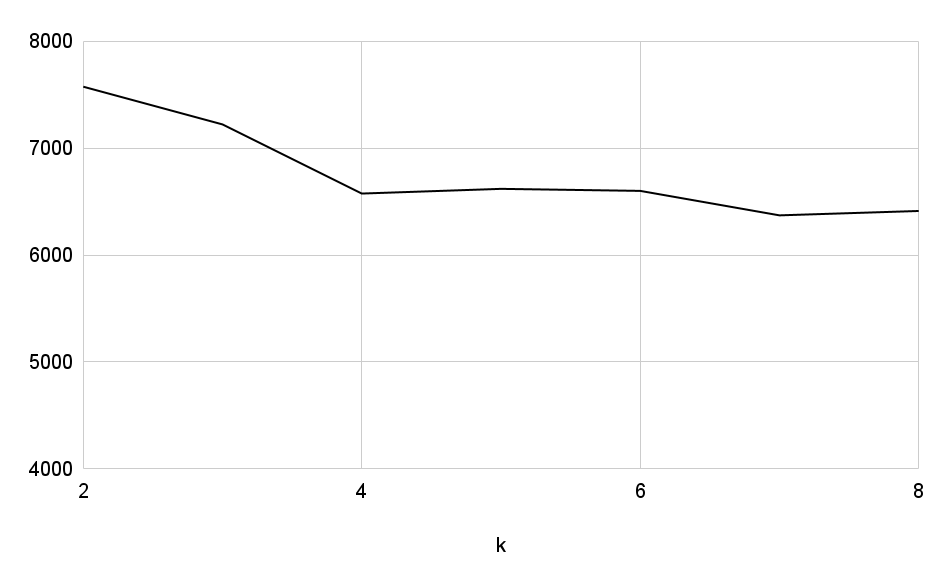
\includegraphics[width=0.7\linewidth]{img/chart.png}
\caption{$k$-means testing loss}
\end{figure}

This indicates an optimal number of clusters of either 3 or 4. The clusters themselves are interesting and deserve some analysis. The paper titles in each cluster for $k = 3$ is listed in appendix A. A scan through the text samples in each cluster reveals some very interesting conclusions. Most notably, there is no clear split of text between different academic disciplines or branches of study. Each cluster contains texts from a wide variety of disciplines and the difference in distribution between each cluster in likely due to random chance.

After manually reading the text within each cluster, it appears that text in the same cluster is written with a similar voice for audiences of similar academic sophistication. In appendix A, we label the clusters with the names \say{high school}, \say{undergrad}, and \say{graduate}, representing this distinction. We therefore conjecture that the distribution of POS transitions may be a good feature for identifying text with similar voice and lexical complexity. Since this conclusion comes from one person's subjective reading of a curated set of text, more work is necessary to come to solid conclusions. As a first start, we describe in section 3.3 a preliminary experiment that explores this conjecture.

\subsection{Markov Models}
We ran a classification task on the genres \textit{learned}, \textit{romance}, \textit{lore}, and \textit{mystery}, reserving 20\% of each genre as a testing set. The results with both the unigram and bigram models are summarized in figure 3.

\begin{figure}[ht!]
\begin{subfigure}[h]{\linewidth}
\centering
\begin{tabular}{|c|c|c|c|c|c|}
\hline
\textit{1-grams} & Learned & Romance & Lore & Mystery & Accuracy\\
\hline
Learned & 14 & 0 & 2 & 0 & 0.875\\
\hline
Romance & 0 & 4 & 0 & 1 & 0.800\\
\hline
Lore & 2 & 0 & 7 & 0 & 0.778\\
\hline
Mystery & 0 & 1 & 0 & 3 & 0.750\\
\hline
\end{tabular}
\subcaption{Classification results with unigram Markov model}
\end{subfigure}

\hfill
\begin{subfigure}[h]{\linewidth}
\centering
\begin{tabular}{|c|c|c|c|c|c|}
\hline
\textit{2-grams} & Learned & Romance & Lore & Mystery & Accuracy\\
\hline
Learned & 13 & 0 & 3 & 0 & 0.813\\
\hline
Romance & 2 & 2 & 0 & 1 & 0.400\\
\hline
Lore & 5 & 1 & 3 & 0 & 0.333\\
\hline
Mystery & 4 & 0 & 0 & 0 & 0.000\\
\hline
\end{tabular}
\subcaption{Classification results with bigram Markov model}
\end{subfigure}
\caption{Classification Results}
\end{figure}

The results for the unigram models are quite good. The model is not as very accurate at distinguishing between the two nonfiction (learned and lore) or fiction (romance and mystery) genres, but appears to have no trouble distinguishing nonfiction from fiction. This supports our hypothesis that word choice and writing style differs markedly between nonfiction and fiction genres.

The results for the bigram model are markedly less stellar. Although one might assume a more powerful model would result in more accurate classification, this does not appear to be the case for this experiment. We propose several explanations for the disparity between prediction and result.

Firstly, the state space is much larger so each matrix is much more sparse. Thus, each row in the matrix is trained on less data and is more likely to suffer from sampling error. In essence, we are training the bigram model on less data so it is less accurate than the unigram model.

Secondly, the likelihood estimation method cannot deal with zeroes in the matrix. In the case that the model has never been trained on a transition, it assigns likelihood 0 to that transition and thus to the text as a whole. Thus, any genre which has values for all of a text's transitions will achieve a higher likelihood, regardless of how similar the text actually is to the genre. This may explain why all of the predictions skew so heavily to \textit{learned}. Due to being trained on more physical text, it is more likely to contain some of the rarer transitions that other models have never seen.

There is unfortunately not a great fix for this problem. We may consider amending the likelihood estimation method to deal with zeroes in a complex way, but this would likely only be a stopgap for this specific corpus and model. Ultimately we simply need to train the model on more text.

\subsection{Non-fiction Genre Discrimination: A Case Study}
In section 3.1 we hypothesize that POS Markov models are useful in distinguishing genres with distinct voices. To test this hypothesis, we attempted to distinguish the \textit{learned} and \textit{news} genres with the unigram Markov model. Though both are nonfiction genres, news reportage has a very distinctive voice that, if we are correct, should allow the model to easily classify the two genres. Figure 4 summarizes our results using a testing set of 20\%.

\begin{figure}[ht!]
\centering
\begin{tabular}{|c|c|c|c|}
\hline
 & Learned & News & Accuracy\\
\hline
Learned & 16 & 0 & 1.000\\
\hline
News & 1 & 7 & 0.875\\
\hline
\end{tabular}
\caption{Learned vs News genres under unigram Markov model}
\end{figure}
The classification is very good, supporting our conjecture. More work is doubtless necessary to come to workable conclusions, but this is a start.

\section{Conclusion and Further Work}
This paper explores a principled approach to genre discrimination. We draw upon work in computational linguistics to create a human-like approach to text classification. Our model is highly explainable and performs decently against the state of the art. Markov transition models on bigrams appear to perform worse than models on unigrams but this is likely due to a lack of training data in our experiment. We suspect that more data will improve performance significantly. Unfortunately, due to time we were unable to find and preprocess a corpus similar enough to the Brown corpus to augment our dataset.

We also conjecture that POS transition models are well-suited to capture voice and lexical complexity. A preliminary experiment supports this conclusion but future work should explore this connection further. In addition, this paper explores temporal connection in a very limited sense. A Markov model \say{forgets} everything immediately after it passes into the past. Gains may be had by using a more sophisticated temporal model, such as a recurrent neural network, but care should be made to maintain explainability.

\begin{appendices}
\section{3-cluster Results}
\begin{tabular}{|ll|}
\hline
\textbf{\say{High school} Cluster} & \\
\hline
Cornell H. Mayer & Radio. Emission of the Moon and Planets\\
\hline
B. J. D. Meeuse & The Story of Pollination\\
\hline
S. Idell Pyle et al. & Onsets, Completions \& Spans\\
\hline
Jacob Robbins et al. & The Thyroid-Stimulating Hormone\\
\hline
J. W. C. Hagstrom et. al. & Debilitating Muscular Weakness\\
\hline
E. Gellhorn & Prolegomena to a Theory of the Emotions\\
\hline
Max F. Millikan \& Donald L. Blackmer, editors & The Emerging Nations\\
\hline
Joyce O. Hertzler & American Social Institutions\\
\hline
Sister Claire M. Sawyer & Some Aspects of Fertility of a Tri-Racial Isolate\\
\hline
Dale L. Womble & Functional Marriage Course for the Already Married\\
\hline
Jesse W. Grimes \& Wesley Allinsmith & Compulsivity, Anxiety \& School Achievement\\
\hline
Ralph Bc Long & The Sentence \& Tts Parts\\
\hline
William O'Connor & Stocks, Wheat \& Pharaohs\\
\hline
Allan J. Braff \& Roger F. Miller & Wage-Price Policies Under Public Pressure\\
\hline
Wallace Mendelson & Justices Black \& Frankfurter\\
\hline
Irving Perluss & Agricultural Labor Disputes in California 1960\\
\hline
Edwin L. Bigelow \& Nancy H. Otis & Manchester, Vermont, A Pleasant Land\\
\hline
Jimmy Ernst & A Letter to Artists of the Soviet Union\\
\hline
I. B. M. Corporation & IBM 7070, Autocoder Reference Manual\\
\hline
Thomas D. McGrath & Submarine Defense\\
\hline
Nat'l Research Council & Directory of Continuing Numerical Data Projects\\
\hline
Harlan W. Nelson & Food Preservation by Ionizing Radiation\\
\hline
W. K. Asbeck & Forces in Coatings Removal Knife Cutting Method\\
\hline
Joel Frados, editor & Survey of Foamed Plastics\\
\hline
Paul J. Dolon \& Wilfrid F. Niklas & Gain \& Resolution of Fiber Optic Intensifier\\
\hline
Rutherford Aris & The Optimal Design of Chemical Reactors\\
\hline
C. J. Savant Jr. \& R. C. Howard & Principles of Inertial Navigation\\
\hline
\end{tabular}

\noindent
\begin{tabular}{|ll|}
\hline
\textbf{\say{Undergrad} Cluster} &\\
\hline
J. F. Vedder & Micrometeorites\\
\hline
M. Yokayama et al & Chemical \& Serological Characteristics\\
\hline
Clifford H Pope & The Ciant Snakes\\
\hline
Kenneth Hoffman \& Ray Kunze & Linear Algebra\\
\hline
Howard J. Parad & Preventive Casework: Problems \& Implications\\
\hline
William H. Ittelson \& Samuel B. Kutash, editors & Perceptual Changes in Psychopathology\\
\hline
Harold Searles & Schizophrenic Communication\\
\hline
H.A. Cleason & Review of African Language Studies\\
\hline
Committee for Economic Development & Distressed Areas in a Growing Economy\\
\hline
James J. O'Leary & The outlook for Interest Rates in 1961\\
\hline
Albert Schreiber et al. & Defense Procurement \& Small Business\\
\hline
Irving L. Horowitz & Philosophy, Science \& the Sociology of Knowledge\\
\hline
Brand Blanshard & The Emotive Theory\\
\hline
Robert A. Futterman & The Future of Our Cities\\
\hline
Allyn Cox & Completing \& Restoring the Capitol Frescos\\
\hline
John H. Schaar & Escape from Authority, Perspectives of Erich Fromm\\
\hline
Katherine G. McDonald & Figures of Rebellion\\
\hline
Samuel Hynes & The Pattern of Hardy's Poetry\\
\hline
Kenneth Rexroth & Disengagament: The Art of the Beat Generation\\
\hline
\end{tabular}

\noindent
\begin{tabular}{|ll|}
\hline
\textbf{\say{Graduate} Cluster} & \\
\hline
R. C. Binder et al. 1961 & Heat Transfer \& Fluid Mechanics Institute\\
\hline
Harry H. Hull & Normal Forces \& Their Thermodynamic Significance\\
\hline
James A. Ibers et al. & Proton Magnetic Resonance Study\\
\hline
John R. Van Wazer, ed. & Phosphorus and Its Compounds\\
\hline
Francis J. Johnston \& John E. Willard & Exchange Reaction Between Cl2 and CCl4\\
\hline
LeRoy Fothergill & Biological Warfare\\
\hline
Richard F McLaughlin et al. & A Study of the Subgross Pulmonary Anatomy\\
\hline
A. N. Nagaraj \& L. M. Black & Localization of Wound-Tumor Virus Antigen\\
\hline
Frederick Mosteller et al. & Probability with Statistical Applications\\
\hline
R. P. Jerrard & Inscribed Squares in Plane Curves\\
\hline
C. R. Wylie, Jr. & Line Involutions in S3\\
\hline
Frank Lorimer & Demographic Information on Tropical Africa\\
\hline
Raymond J. Corsini & Roleplaying in Business \& Industry\\
\hline
Hugh Kelly \& Ted Ziehe & Glossary Lookup Made Easy\\
\hline
A. T. Kroeber & Semantic Contribution of Lexicostatistics\\
\hline
D. F. Fleming & The Cold War \& Its Origins\\
\hline
Douglas Ashford & Elections' in Morocco: Progress or Confusion\\
\hline
Morton A. Kaplan \& Nicholas Katzenbach & The Political Foundation of Internationa1 Law\\
\hline
J. Mitchell Reese, Jr, & Reorganization Transfers\\
\hline
William S. Ragan & Teaching America's Children.\\
\hline
Paul Cooke & Desegregated Education in the Middle-South Region\\
\hline
Robert J. Havighurst & Social-Class Influences on American Education\\
\hline
James C. Bonbright & Principles of Public Utility Rates\\
\hline
William S. Haymond & Is Distance an Original Factor in Vision?\\
\hline
Chester G. Starr & The Origins of Greek Civilization 1100-650 B. C\\
\hline
Jim B. Pearson & The Maxwell Land Grant\\
\hline
J. H. Hexter & Thomas More: on the Margins of Modernity\\
\hline
John M, Ray & Rhode Island's Reactions to John Brown's Raid\\
\hline
Clement Greenberg & Collage\\
\hline
William Whallon & The Diction of Beowulf\\
\hline
Charles R. Forker & The Language of Hands in Great Expectations\\
\hline
Ross E. McKinney \& Howard Edde & Aerated Lagoon for Suburban Sewage Disposal\\
\hline
Mellon Institute & Annual Report; 1960, Independent Research\\
\hline
William D. Appel, editor & 1961 Technical Manual of American Ass'n of Textile\\
 & Chemists \& Colorists\\ % page break
\hline
\end{tabular}
\end{appendices}

\bibliography{report}

\end{document}

% List of tex snippets:
%   - tex-header (this)
%   - R      --> \mathbb{R}
%   - Z      --> \mathbb{Z}
%   - B      --> \mathcal{B}
%   - E      --> \mathbb{E}
%   - M      --> \mathcal{M}
%   - m      --> \mathfrak{m}({#1})
%   - normlp --> \norm{{#1}}_{L^{{#2}}}
%   - dd     --> \;\mathrm{d}{#1}
